Như đã đề cập từ các phần trước, hệ thống hỗ trợ quyết định được mô hình hóa dựa trên mô hình Ikigai. Theo sơ đồ Venn Ikigai, một Ikigai - lý do để sống của mỗi người - là giao điểm của 4 câu hỏi: Bạn thích điều gì? Bạn giỏi điều gì? Điều gì mang lại thu nhập cho bạn? Và điều gì thế giới cần? Đối với một người, việc thật sự trả lời được 4 câu hỏi này và tìm được giao điểm chung của chúng quả thật là khó khăn và vất vả. Trong hệ thống này, chúng tôi cũng sẽ đi trả lời lần lượt 4 câu hỏi trên để tìm kiếm Ikigai - lý do để thức dậy mỗi buổi sáng của mỗi người.

Bạn thích điều gì? Để trả lời cho câu hỏi này, đồ án sử dụng phương pháp đánh giá MBTI. Mối quan hệ giữa việc yêu thích và nghề nghiệp được nói vô cùng chi tiết thông qua cuốn \textit{Type Talk: The 16 Personality Types That Determine How We Live, Love, and Work} của Otto Kroeger và Janet M.Thunes.

Bạn giỏi điều gì? Để trả lời cho câu hỏi này, nhóm sử dụng phương pháp Career Interest Clustering đã được nêu ở \hyperref[2]{phần 2} và cách đánh giá chi tiết tại \hyperref[3.3]{phần 3.3}.

Điều gì mang lại thu nhập cho bạn? Sử dụng cơ sở dữ liệu về tiền lương và việc làm được mô tả chi tiết ở \hyperref[3.1]{phần 3.1}.

Điều gì thế giới cần? Sử dụng cơ sở dữ liệu về ngành nghề và số lượng lao động được mô tả chi tiết ở \hyperref[3.1]{phần 3.1}.

Sau khi tổng hợp dữ liệu, nhóm sử dụng các thuật toán MCDM để đánh giá các giải pháp và đưa ra gợi ý dựa trên giải pháp tốt nhất. Thuật toán được lựa chọn trong mô hình lần này là VIKOR và Weighted Sum.

\begin{figure}[H]
    \centering
    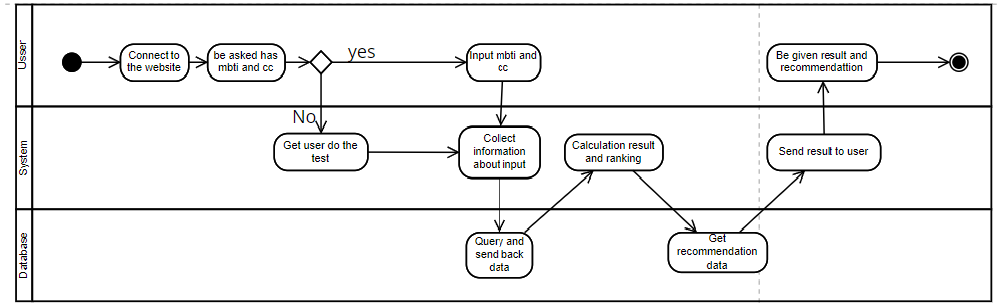
\includegraphics[width=0.8\linewidth]{images/chap3/activity.png}
    \vspace{0.5cm}
    \caption{Sơ đồ activyty diagram - sơ đồ hoạt động chính của thuật toán}
\end{figure}

\import{chapters/3. Phương pháp thực hiện/}{3.1. Xây dựng hệ cơ sở dữ liệu.tex}

\import{chapters/3. Phương pháp thực hiện/}{3.2. Thu thập, đánh giá MBTI từ người dùng.tex}

\import{chapters/3. Phương pháp thực hiện/}{3.3. Thu thập phân cụm người dùng từ Career Interest Clustering.tex}

\import{chapters/3. Phương pháp thực hiện/}{3.4. Tính toán và xếp hạng kết quả.tex}

\import{chapters/3. Phương pháp thực hiện/}{3.5. Các bài kiểm tra khác.tex}